\section{Einführung}

\begin{frame}{Disclaimer}
  \begin{itemize}
    \item dieser Kurs ist \enquote{opinionated} (habe keine passende Übesetzung gefunden…)
    \item in \LaTeX\ gibt es immer viele Möglichkeiten, ein Ziel zu erreichen
    \item wir zeigen eine der Möglichkeiten, nämlich die, die wir am besten finden
    \item wir erklären, warum wir diese Möglichkeit gewählt haben
    \item wir zeigen am Rand einige wichtige Alternativen, damit man sie erkennt
  \end{itemize}

  \vspace{10pt}
  \begin{itemize}
    \item Inhalt anders als in früheren Jahren
    \item Zeit reicht nicht, um alle veralteten Alternativen zu zeigen
  \end{itemize}
\end{frame}

\begin{frame}{Was ist \LaTeX?}
  \begin{itemize}
    \item \emph{Programmiersprache} zum Setzen von Text
    \item Kein WYSIWYG, es werden Befehle und Inhalt in normale Text-Dateien geschrieben.
    \item Kompiler überträgt \LaTeX-Code in ein Ausgabedokument (meist PDF)
    \item open-source mit zahlreichen Erweiterungsmöglichkeit (Pakete)
  \end{itemize}
\end{frame}

\begin{frame}{Warum \LaTeX?}
  \begin{itemize}
    \item hervorragender Text- und Formelsatz
    \item automatisierte Erstellung von Inhalts- und Literaturverzeichnis
      \begin{itemize}
        \item und anderen Verzeichnissen: Index, Glossar, Abkürzungen, Definitionen, …
      \end{itemize}
    \item \TeX-Dateien sind reine Text-Dateien
      \begin{itemize}
        \item[$\Rightarrow$] gut für Versionskontrolle geeignet
      \end{itemize}
    \item sehr gute Vorlagen für wissenschaftliches Arbeiten
    \item aber auch: Briefe, Notensatz, Präsentationen (auch diese)
    \item ausgezeichnete Dokumention
    \item erweiterbar durch zahlreiche und mächtige Pakete
    \item auf allen geläufigen Betriebssystemen verfügbar
    \item Ausgabe direkt als PDF mit Hyperlinks
  \end{itemize}
\end{frame}

\begin{frame}{Geschichte}
  \begin{columns}
    \begin{column}{0.75\textwidth}
      \TeX:
      \begin{itemize}
        \item Geschrieben von Donald E. Knuth 1978, um sein Buch \enquote{The Art of Computer Programming} zu setzen
        \item auf Aussprache achten!
        \item Version (2014) $3.14159265 → \mathup{π}$
        \item viele Erweiterungen: \eTeX, pdf\TeX, \XeTeX, \LuaTeX
      \end{itemize}

      \vspace{10pt}
      \LaTeX:
      \begin{itemize}
        \item Geschrieben von Leslie Lamport 1984
        \item Version (1994) \LaTeXe
        \item \LaTeX3 seit Anfang der Neunziger in Arbeit…
      \end{itemize}
    \end{column}
    \begin{column}{0.25\textwidth}
      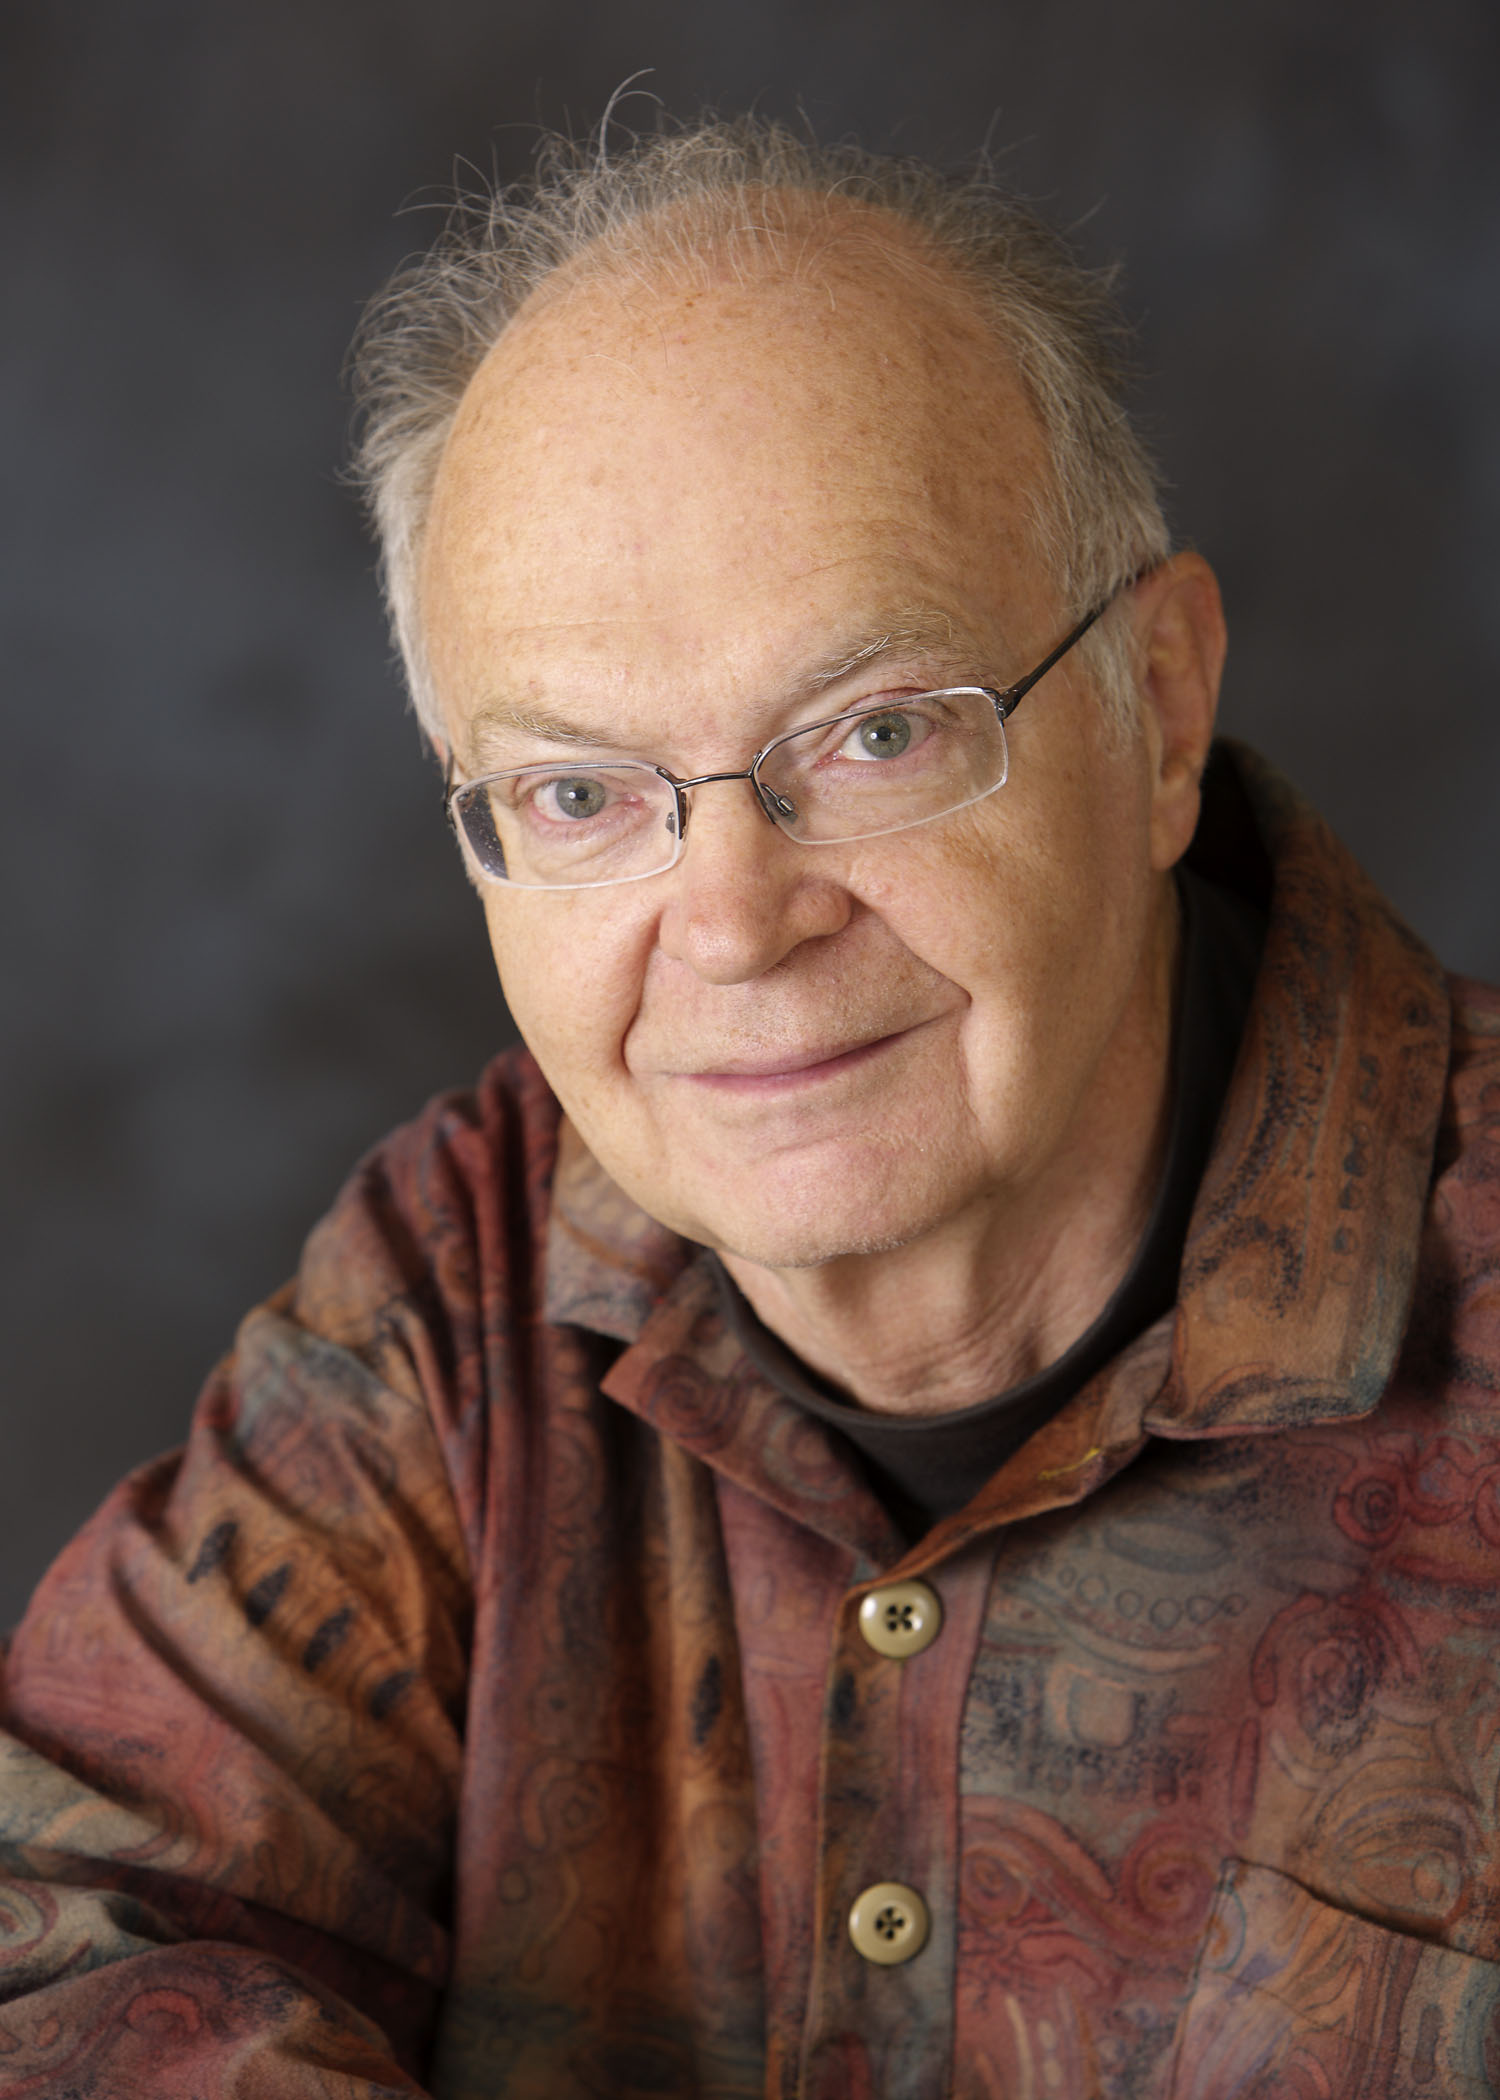
\includegraphics[height=0.45\textheight]{figures/knuth.jpg}\\
      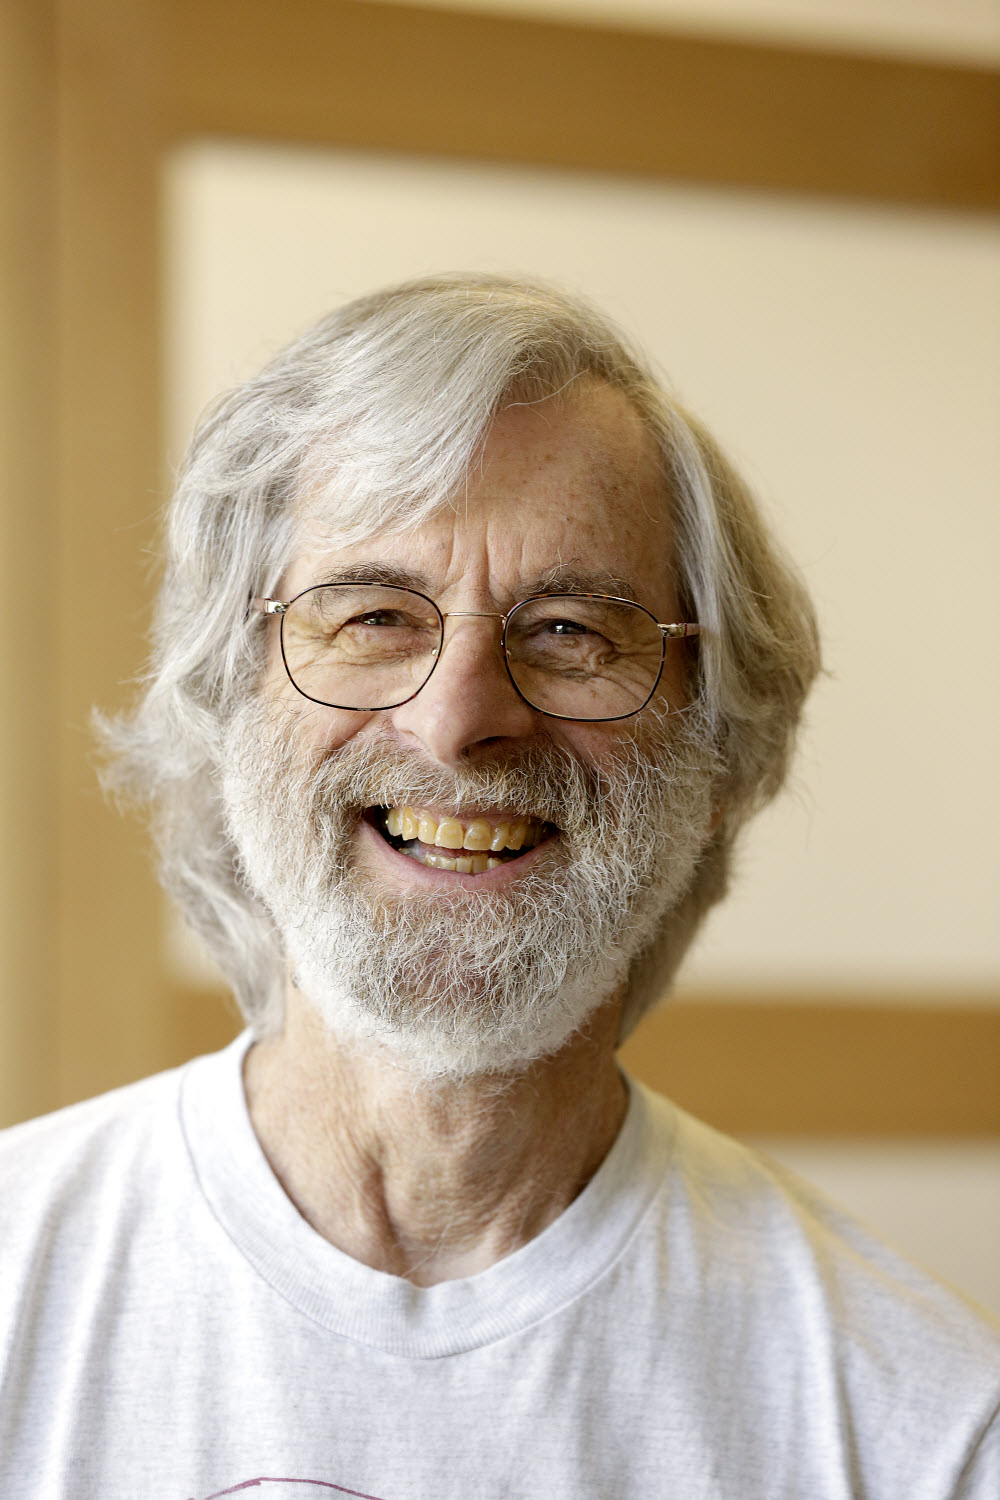
\includegraphics[height=0.45\textheight]{figures/lamport.jpg}
    \end{column}
  \end{columns}
\end{frame}

\begin{frame}{Begriffe}
  \begin{description}
    \item[\TeX-Engine] Implementierung von \TeX, wird als Programm ausgeführt
    \item[\TeX-Format] Paket, welches standardmäßig geladen wird, z.B. \LaTeX
  \end{description}

  \vspace{10pt}
  Eine Kombination davon ist oft ein neues Programm.\\[10pt]
  Beispiel: \texttt{dvilualatex} = \LuaTeX + \LaTeX + DVI-Output (statt PDF)
\end{frame}

\begin{frame}
  \centering
  \only<1>{
    \includegraphics[height=0.95\textheight]{figures/engines-few.pdf}
    \hspace{1.15em}
  }
  \only<2,3>{
    \includegraphics[height=0.95\textheight]{figures/engines-many.pdf}
  }
  \begin{tikzpicture}[remember picture,overlay]
    \tikzset{shift={(current page.center)}}
    \node at (-4.3,1.3) {
      \TeX-Engines
    };
    \only<3>{
      \node (here) at (-4.3,-2.8) {
        Sie sind hier
      };
      \draw [->, >=Stealth] (here.east) -- ++(1.55,-0.85);
    }
  \end{tikzpicture}
\end{frame}

\begin{frame}[fragile]{Warum \LuaTeX?}
  \begin{itemize}
    \item Unicode-Input
      \begin{itemize}
        \item Bequem, äöüßêéè funktioniert einfach
      \end{itemize}
    \item OTF-Fonts
      \begin{itemize}
        \item Alle Fonts benutzen, die man auf dem Rechner hat (heißt nicht, dass man das tun sollte…)
      \end{itemize}
    \item Unicode-Math
      \begin{itemize}
        \item Mathe-Input über Unicode (bei mir: <Caps><Caps>a → $α$)
          \begin{itemize}
            \item Code lesbarer, Tippen schneller
            \end{itemize}
        \item Mehr Font-Möglichkeiten
          \begin{itemize}
            \item Umsetzung von ISO 80000-1
          \end{itemize}
      \end{itemize}
    \item Lua-Programmierung
      \begin{itemize}
        \item \TeX-Programmierung ist nicht besonders einfach
        \item manche Pakete bieten komplizierte Funktionen nur über Lua an
          \begin{itemize}
            \item Graph-Layout von Ti\emph{k}Z (übrigens \emph{kein} Zeichenprogramm)
          \end{itemize}
      \end{itemize}
  \end{itemize}
\end{frame}

\begin{frame}[t]
  \centering
  \only<1>{
    \includegraphics[height=5.45em]{figures/formats-few.pdf}
    \hspace{0.5em}
  }
  \only<2,3>{
    \includegraphics[height=0.95\textheight]{figures/formats-many.pdf}
  }
  \begin{tikzpicture}[remember picture,overlay]
    \tikzset{shift={(current page.center)}}
    \node at (-4.3,2.5) {
      \TeX-Formate
    };
    \only<3>{
      \node (here) at (-4.3,-0.6) {
        Sie sind hier
      };
      \draw [->, >=Stealth] (here.east) -- ++(3.05,0);
    }
  \end{tikzpicture}
\end{frame}

\begin{frame}{Warum \LaTeX3?}
  \begin{itemize}
    \item \LaTeX3 existiert (noch) nicht
    \item \texttt{expl3} ist \LaTeX3 unter \LaTeXe
    \item \texttt{xpackages} sind Pakete, die auf \texttt{expl3} aufbauen und neue Möglichkeiten bieten
    \item \texttt{xparse} macht das schreiben neuer (auch komplizierter) Befehle sehr einfach
    \item viele Pakete benutzen jetzt schon \texttt{expl3} und \texttt{xparse}
  \end{itemize}
\end{frame}
